\documentclass{article}
\usepackage[utf8]{inputenc}
\usepackage[margin=1.2in]{geometry}
\usepackage{hyperref}

\usepackage{listings}
\usepackage{xcolor}

\definecolor{codegreen}{rgb}{0,0.6,0}
\definecolor{codegray}{rgb}{0.5,0.5,0.5}
\definecolor{codepurple}{rgb}{0.58,0,0.82}
\definecolor{backcolour}{rgb}{.95,.95,.95}

\lstdefinestyle{mystyle}{
    backgroundcolor=\color{backcolour},   
    commentstyle=\color{codegreen},
    %keywordstyle=\color{magenta},
    numberstyle=\tiny\color{codegray},
    %stringstyle=\color{codepurple},
    %basicstyle=\ttfamily\footnotesize,
    breakatwhitespace=false,         
    breaklines=true,                 
    captionpos=b,                    
    keepspaces=true,                 
    numbers=left,                    
    numbersep=5pt,                  
    showspaces=false,                
    showstringspaces=false,
    showtabs=false,                  
    tabsize=2
}

\lstset{style=mystyle}


\usepackage{tikz}
\usetikzlibrary{positioning}

\usepackage{natbib}
\usepackage{graphicx}
\usepackage{amsmath}

\title{\vspace{-2 cm} PCC104 - Projeto e Análise de Algoritmos}
%\author{}
%\date{}


\begin{document}

\maketitle

Orientações:
\begin{itemize}
    \item É obrigatória a entrega do código fonte dos algoritmos implementados. Provas sem os códigos fonte não serão corrigidas e terão nota 0.
    \item O código não deve conter nenhuma informação/comentário que auxilie na análise de complexidade do mesmo.  
    \item Simplificações feitas na análise de custo dos algoritmos devem ser indicadas e justificadas.
\end{itemize}

\section*{Questões}

\begin{enumerate}

    \item Quando devemos utilizar programação dinâmica?
   
    \item Considere a sua implementação do algoritmo que resolve o \textit{coin-collecting problem} e a instância apresentada na Figura \ref{fig:coin_col} :
    
    \begin{figure}[!ht]
        \centering
        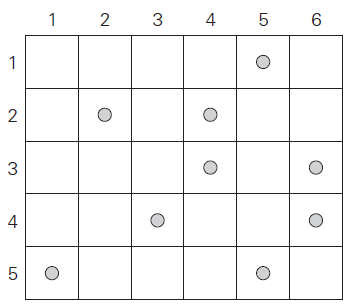
\includegraphics[width=0.4\textwidth]{tabCoinColl.png}
        \caption{Coin-collecting problem instance}
        \label{fig:coin_col}
    \end{figure}

    \begin{enumerate}
        \item Apresente o resultado do algoritmo de programação dinâmica, ou seja, como a estrutura de memória fica ao final da execução.
        \item Baseado na solução apresentada, mostre o caminho em que pode-se coletar o maior número de moedas possível. 
        \item Apresente a análise completa do custo do seu algoritmo de programação dinâmica.
    \end{enumerate}

    \item Considere o problema \textit{Change Making} em sua versão de decisão, ou seja: ``Dadas moedas de denominação $d_1 < d_2 < ... <d_m$ existe uma forma de dar o troco de valor $n$ com menos do que $k$ moedas'':
    \begin{enumerate}
        \item Este é um problema da classe $P$, $NP$ ou $NP-completo$? Explique.
        \item Como eu posso provar que este problema é da classe $NP$?
        \item Seu eu quisesse tentar provar que este problema pertence à classe $NP-completo$ o que eu deveria fazer?
    \end{enumerate}
   
\end{enumerate}



%\bibliographystyle{plain}
%\bibliography{references}
\end{document}
